\documentclass[10pt]{article}

\usepackage[a4paper, left=2cm, right=2cm]{geometry} % A4 paper size and thin margins

\usepackage{xcolor} % Required for specifying custom colours
\definecolor{grey}{rgb}{0.9,0.9,0.9} % Colour of the box surrounding the title

\usepackage{graphicx}
\usepackage[colorlinks=true, allcolors=black]{hyperref}
\usepackage{amsmath}
\usepackage{indentfirst}
\usepackage{subfigure}
\setlength{\parindent}{2em}

\usepackage[utf8]{inputenc} % Required for inputting international characters
\usepackage[T1]{fontenc} % Output font encoding for international characters
\usepackage[sfdefault]{ClearSans} % Use the Clear Sans font (sans serif)
%\usepackage{XCharter} % Use the XCharter font (serif)
\usepackage{float}

\newcommand{\tabincell}[2]{\begin{tabular}{@{}#1@{}}#2\end{tabular}} 	

\begin{document}
%----------------------------------------------------------------------------------------
%	TITLE PAGE
%----------------------------------------------------------------------------------------

\begin{titlepage} % Suppresses displaying the page number on the title page and the subsequent page counts as page 1
	
	%------------------------------------------------
	%	Grey title box
	%------------------------------------------------
	
	\colorbox{grey}{
		\parbox[t]{1.1\textwidth}{ % Outer full width box
			\parbox[t]{1.02\textwidth}{ % Inner box for inner right text margin
				\raggedleft % Right align the text
				\fontsize{34pt}{40pt}\selectfont % Title font size, the first argument is the font size and the second is the line spacing, adjust depending on title length
				\vspace{0.7cm} % Space between the start of the title and the top of the grey box
				
				< Journey Assistant >\\
                User Manual\\
                Version 1.0\\
				
				\vspace{0.7cm} % Space between the end of the title and the bottom of the grey box
			}
		}
	}
	
	\vfill % Space between the title box and author information
	
	%------------------------------------------------
	%	Author name and information
	%------------------------------------------------
	
	\parbox[t]{1\textwidth}{ % Box to inset this section slightly
		\raggedleft % Right align the text
		\large % Increase the font size
		{\Large Group Member}\\[4pt] % Extra space after name
        Yiwen Song\\
        Zhihui Xie\\
        Weizhe Wang\\
        Huangfei Jiang\\
        Haoping Chen\\
		% Institution Name\\[4pt] % Extra space before URL
		% \texttt{LaTeXTemplates.com}\\
		
		\hfill\rule{0.2\linewidth}{1pt}% Horizontal line, first argument width, second thickness
    }
    
	
\end{titlepage}

\newpage

\begin{center}
    {\LARGE Modification History}
    
    \begin{tabular}{|c|c|c|c|} 
        \hline 
        Date&Version&Description&Author\\
        \hline  
        2019-06-18&1.0&Finish the first version.&Huangfei Jiang\\
		\hline 
		& & & \\
		\hline
		& & & \\
		\hline
		& & & \\
		\hline
    \end{tabular}    
\end{center}

\newpage

\tableofcontents
\newpage

\section{Intruduction}
\subsection{Purpose}
The purpose of this user manual is to explain the use and operation of Journey Assistant software. In the manual, the function of the software is introduced, the operating environment is specified, and the operating process and steps are explained in detail. This document is used to assist users to use the software smoothly.

\subsection{Scope}
Scope of application software applicable to this document:Journey Assistant Software.The features, subsystems, models, and code associated with the software conform to this document.

\subsection{Definition}
The terms referred to in this document are defined in the project glossary document (Glossary.pdf).

\subsection{Bibliography}
\begin{itemize}
	\item[1.] <Object Oriented Software Engineering (Version 3)> (Tsinghua University Press)
	\item[2.] <Object Oriented Software Engineering Practice Guidelines> 
\end{itemize}

\subsection{Sketch}
This user manual includes four parts: software overview, operating environment, operating process and operating instructions.The software overview section describes the composition and functions of the software. The operating environment section defines the environment in which the software is used. The usage process introduces the usage method of the software in detail by steps. The operating instructions describe the operating steps of the system.The various parts of this document are closely related and describe in detail the situation and use of the software. Each part complements and contrasts with each other to guide users' use.

\section{Software Overview}
This section is reproduced from the Software Acceptance Report, hence it is omitted here.

\section{Operating Environment}
\subsection{Hardware Environment}
\paragraph{\underline{Server}}
\subparagraph{Processor}
AMDA4 5000M, Intel core I 53210m or above.

\subparagraph{Memory}
4GBDDR3 or above.

\subparagraph{External Storage}
1× 500GB HDD or better configuration.

\subparagraph{Network Environment}
WAN connection with 10Mbps or above.

\paragraph{\underline{Client}}
\subparagraph{Processor}
ARM cortex-A91GHz dual-core or above.

\subparagraph{Memory}
512MB or above.

\subparagraph{External Storage}
512MB or above.

\subparagraph{Network Environment}
2G / 3G / 4G / WiFI network access.

\subsection{Supporting Software}
\paragraph{\underline{Server}}
\begin{itemize}
	\item Microsoft Windows 7/10.
	\item JAVA 8 update 91 64bit.
	\item SQLite 3.
	\item Apache tomcat 9.0.20
\end{itemize}

\paragraph{\underline{Client}}
Android 4.4 or above.

\subsection{Data Structure}
This project uses a relational database, specifically SQLite3. In fact, it is the same physical machine as the server.

\section{Use Process}
\subsection{Installation and Initialization}
\begin{itemize}
	\item The client first needs to get the installation package (.Apk file), open the installation package, and the software installation is completed.
	\item Unzip the compressed file on the server side, put it in the root directory of a disk, open any IDE you like, import project, and run the project in the form of JAVA server.
\end{itemize}

\subsection{Input}
\subsubsection{Input for Registration}
\paragraph{\underline{Name}}
A string of characters, which can be numbers, letters, and symbols, of at least 4 digits in length. Example: jhf1234.

\paragraph{\underline{Mail}}
A legal mailbox address string. Example:JiangHF123@qq.com. 

\paragraph{\underline{Password}}
A string of characters, which can be numbers, letters, and symbols, of at least 4 digits in length. Example: abcd1234.

\subsubsection{Input for Login}
\paragraph{\underline{Mail}}
A legal mailbox address string. Example:JiangHF123@qq.com. 

\paragraph{\underline{Password}}
A string of characters, which can be numbers, letters, and symbols, of at least 4 digits in length. Example: abcd1234.

\subsubsection{Input for Feedback}
\paragraph{\underline{Description}}
A string of characters, which can be numbers, letters, and symbols, of at least 4 digits in length. Example: "There are bugs everywhere!".

\subsubsection{Output}
Output when the software is running, all results of interaction with users are output in the form of interface interaction, which does not contain a large amount of formatted data. Therefore, please refer to the operation instructions for the operation steps.

\subsection{Help Information Acquisition}
Please contact the developer if you encounter any problems during the operation of help information acquisition.

Developer email: JiangHF123@qq.com.

\section{Operating Instruction}
\subsection{Operating Steps}
\subsubsection{Register}
New user should apply an account with which he could get the ID in this application.

\subsubsection{Login}
Enter username and password as instruction held above.

\begin{figure}[H]
	\centering
	\subfigure[Login]{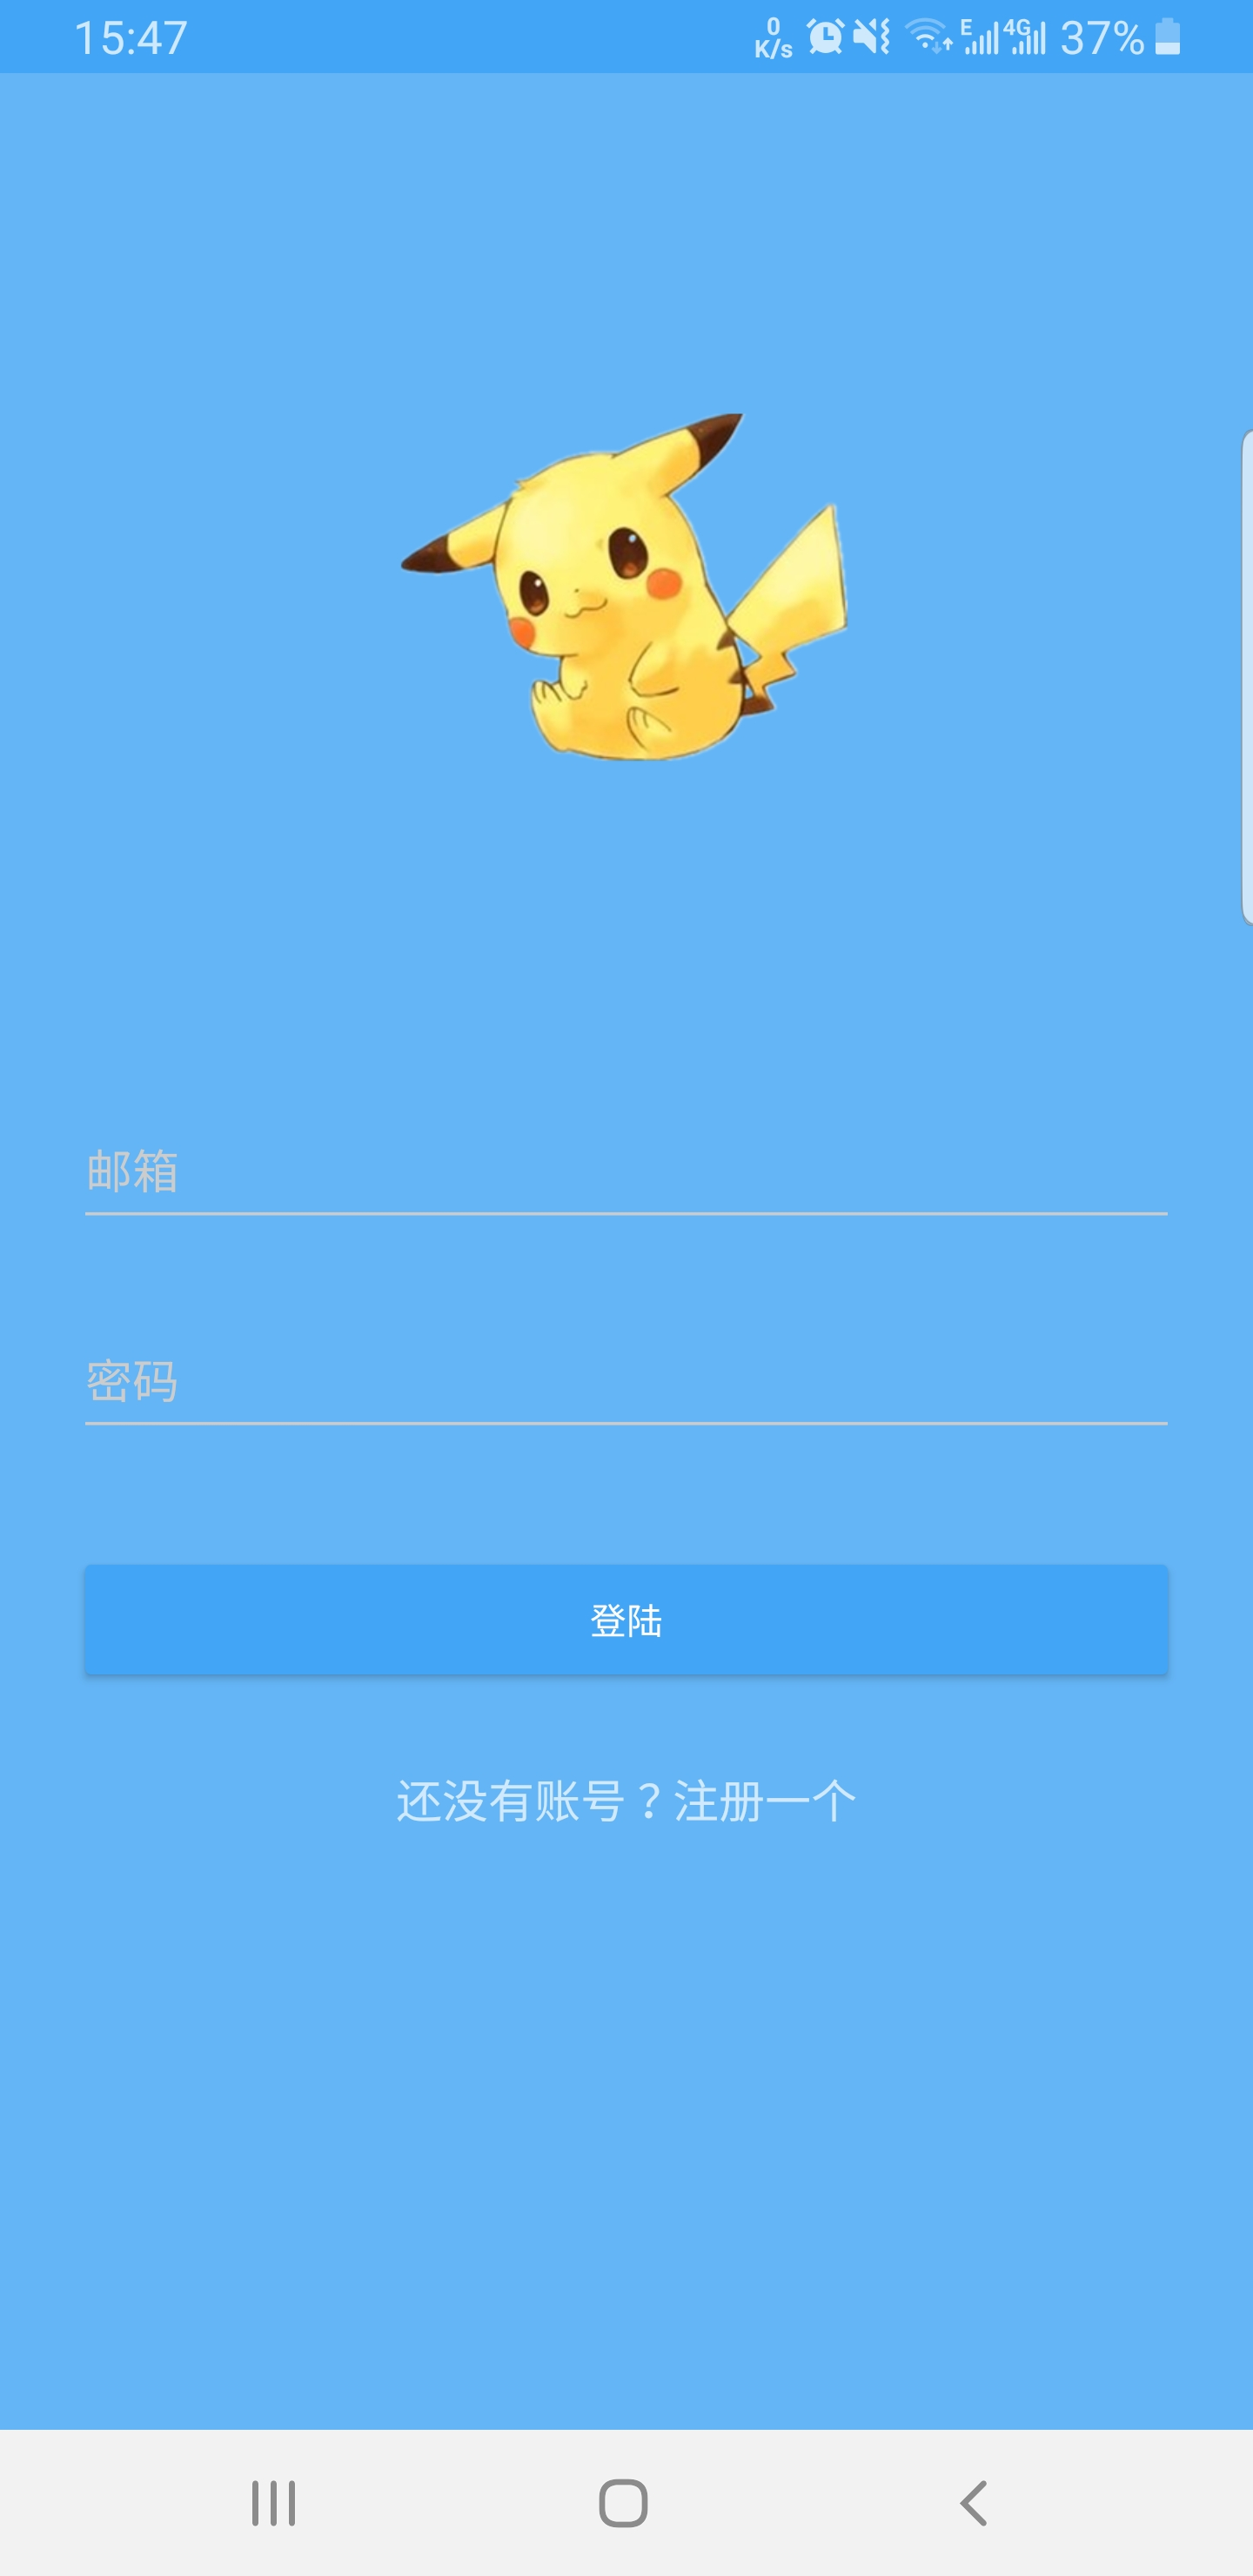
\includegraphics[width=6cm]{login.jpg}}
	\quad
	\subfigure[Register]{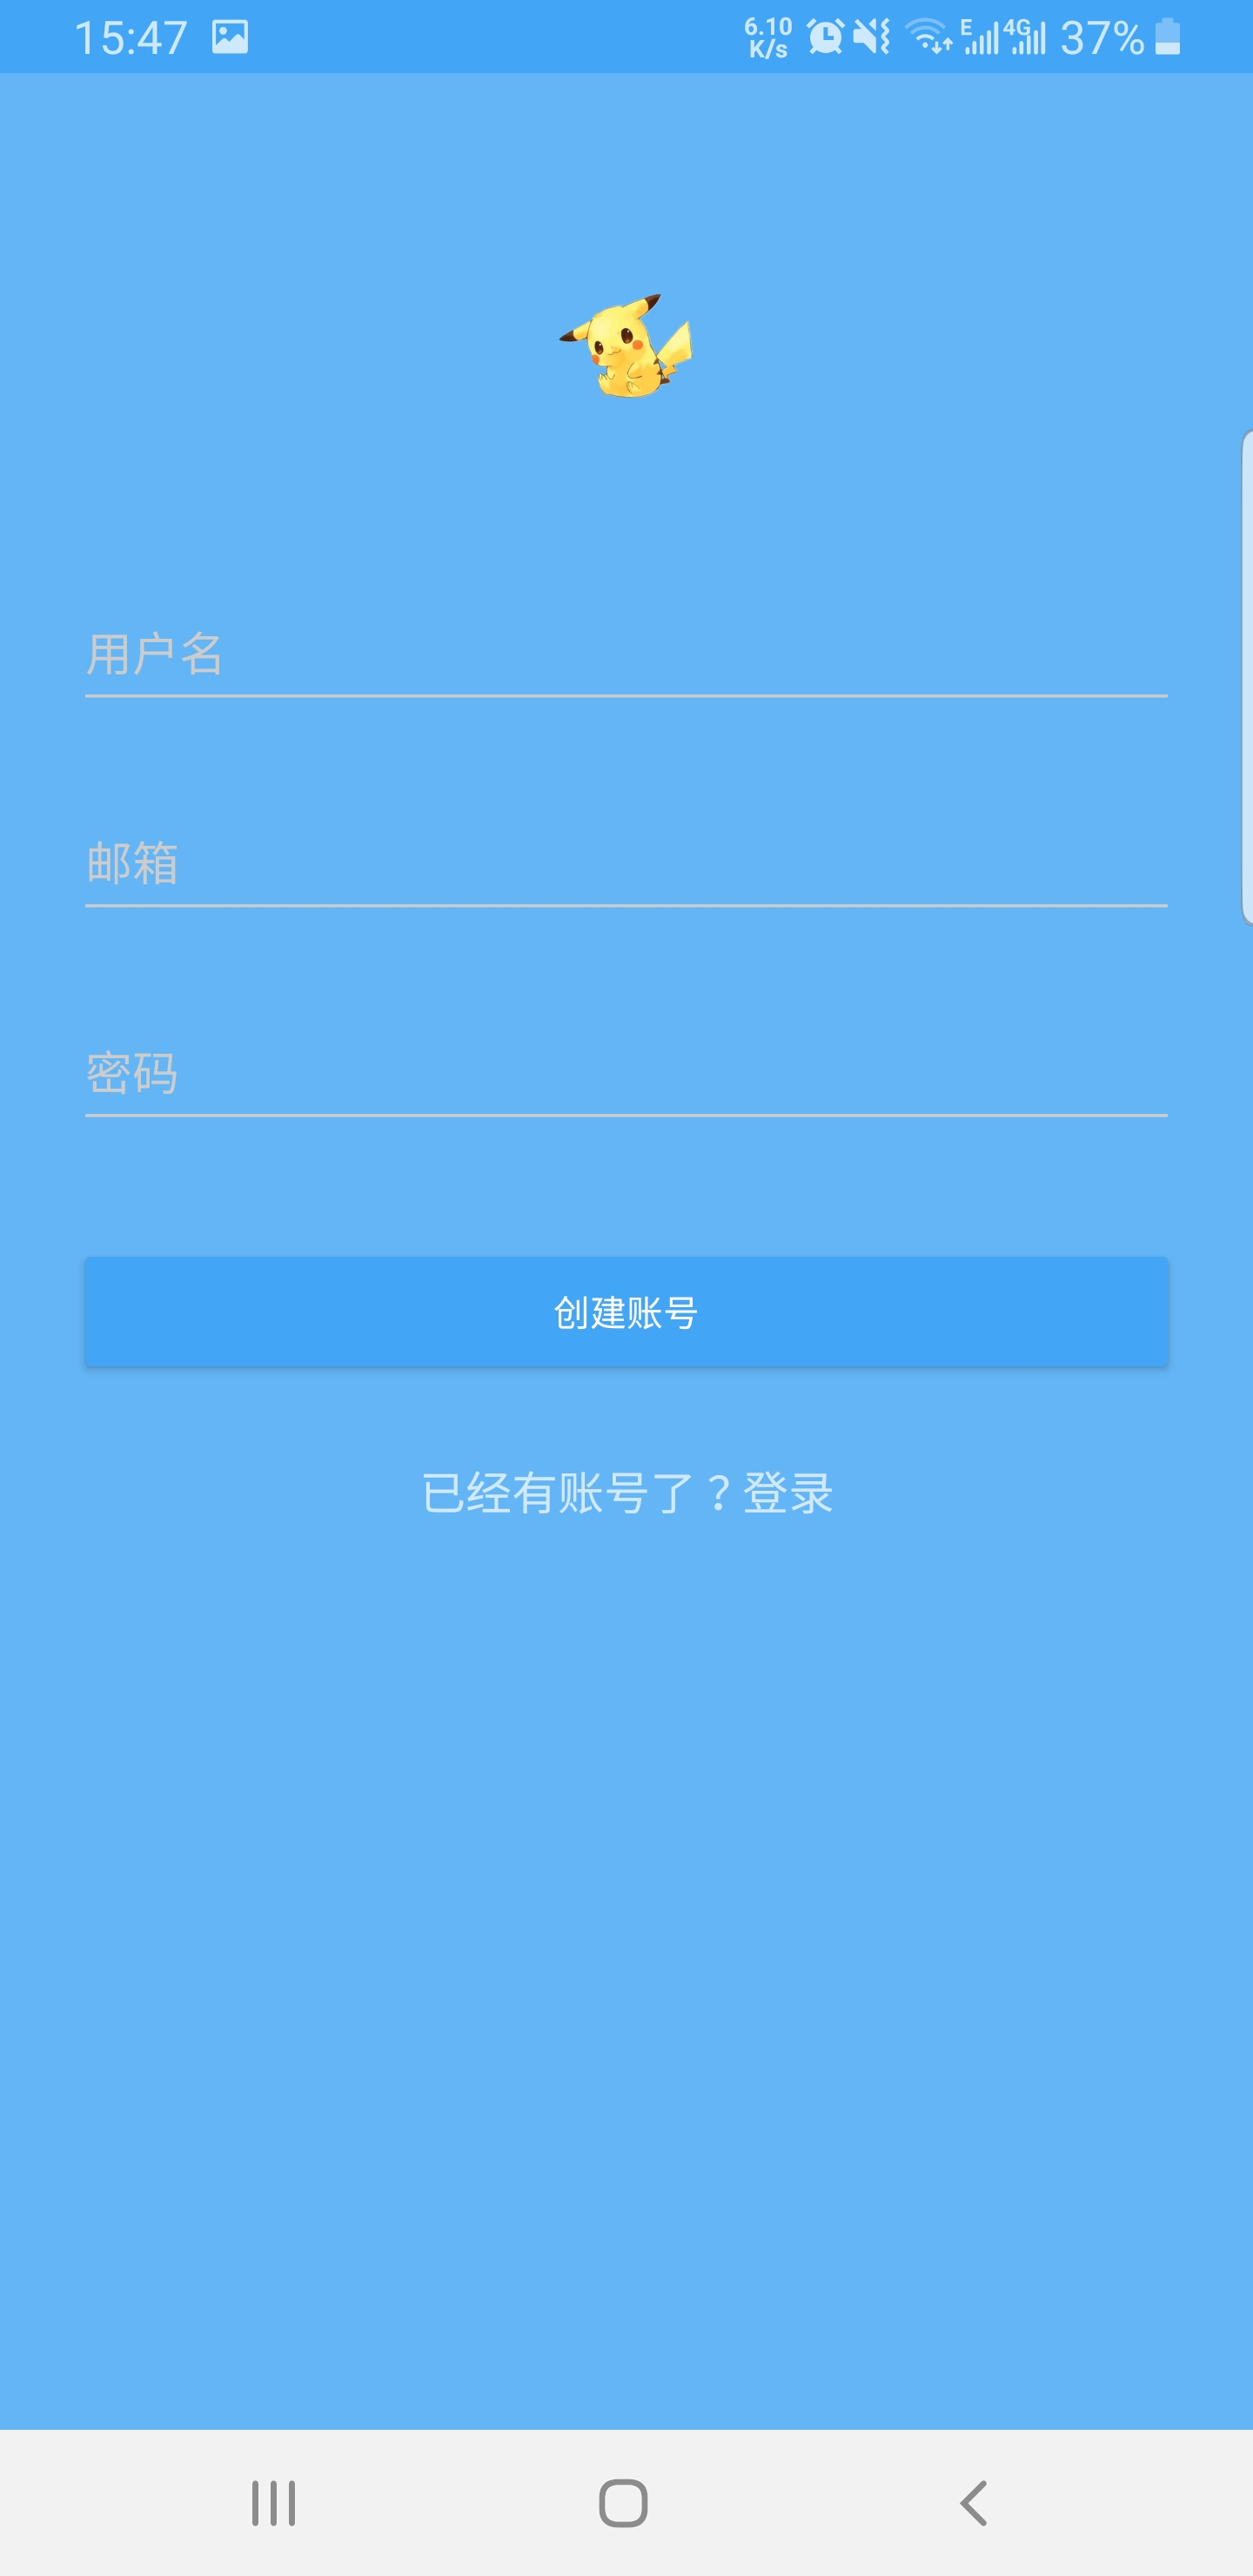
\includegraphics[width=6cm]{register.jpg}}

	% \caption{Login}
	% \label{Login}
\end{figure}

\subsubsection{Select Destination}
Choose one city you like to travel in. The message held in the top right corner shows temperature in corresponding city while description below the city’s basic information offers weather recommendation message.

\subsubsection{Select Mode}
Choose the mode you prefer.

\begin{figure}[H]
	\centering
	\subfigure[Select Destination]{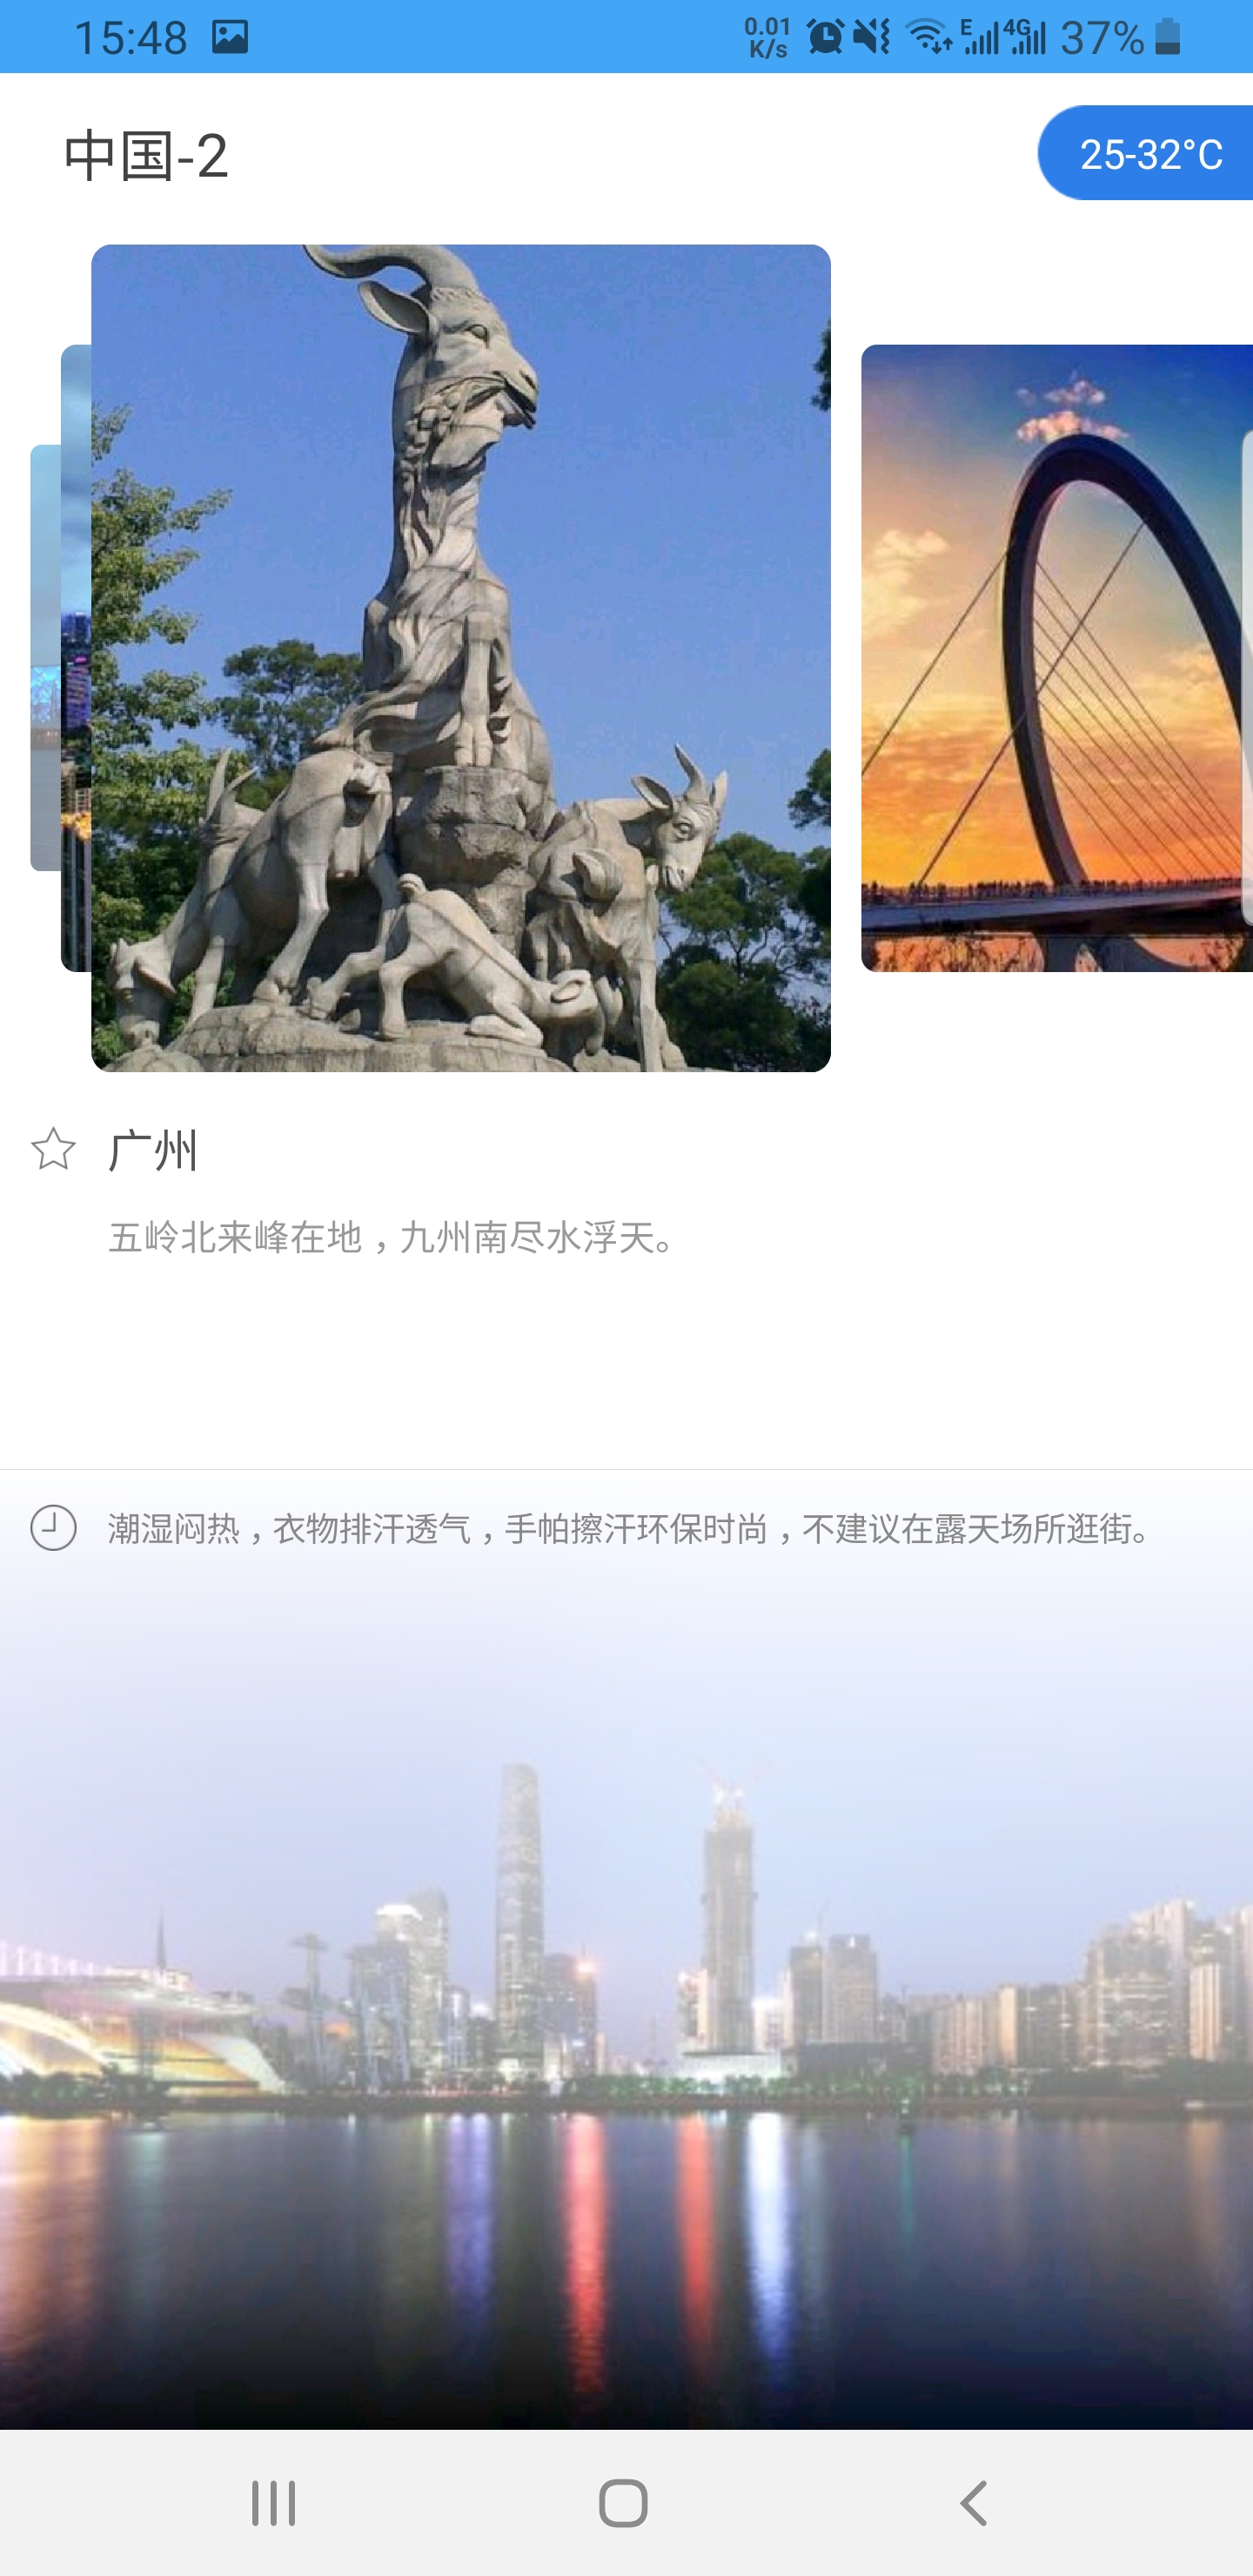
\includegraphics[width=6cm]{destination.jpg}}
	\quad
	\subfigure[Select Mode]{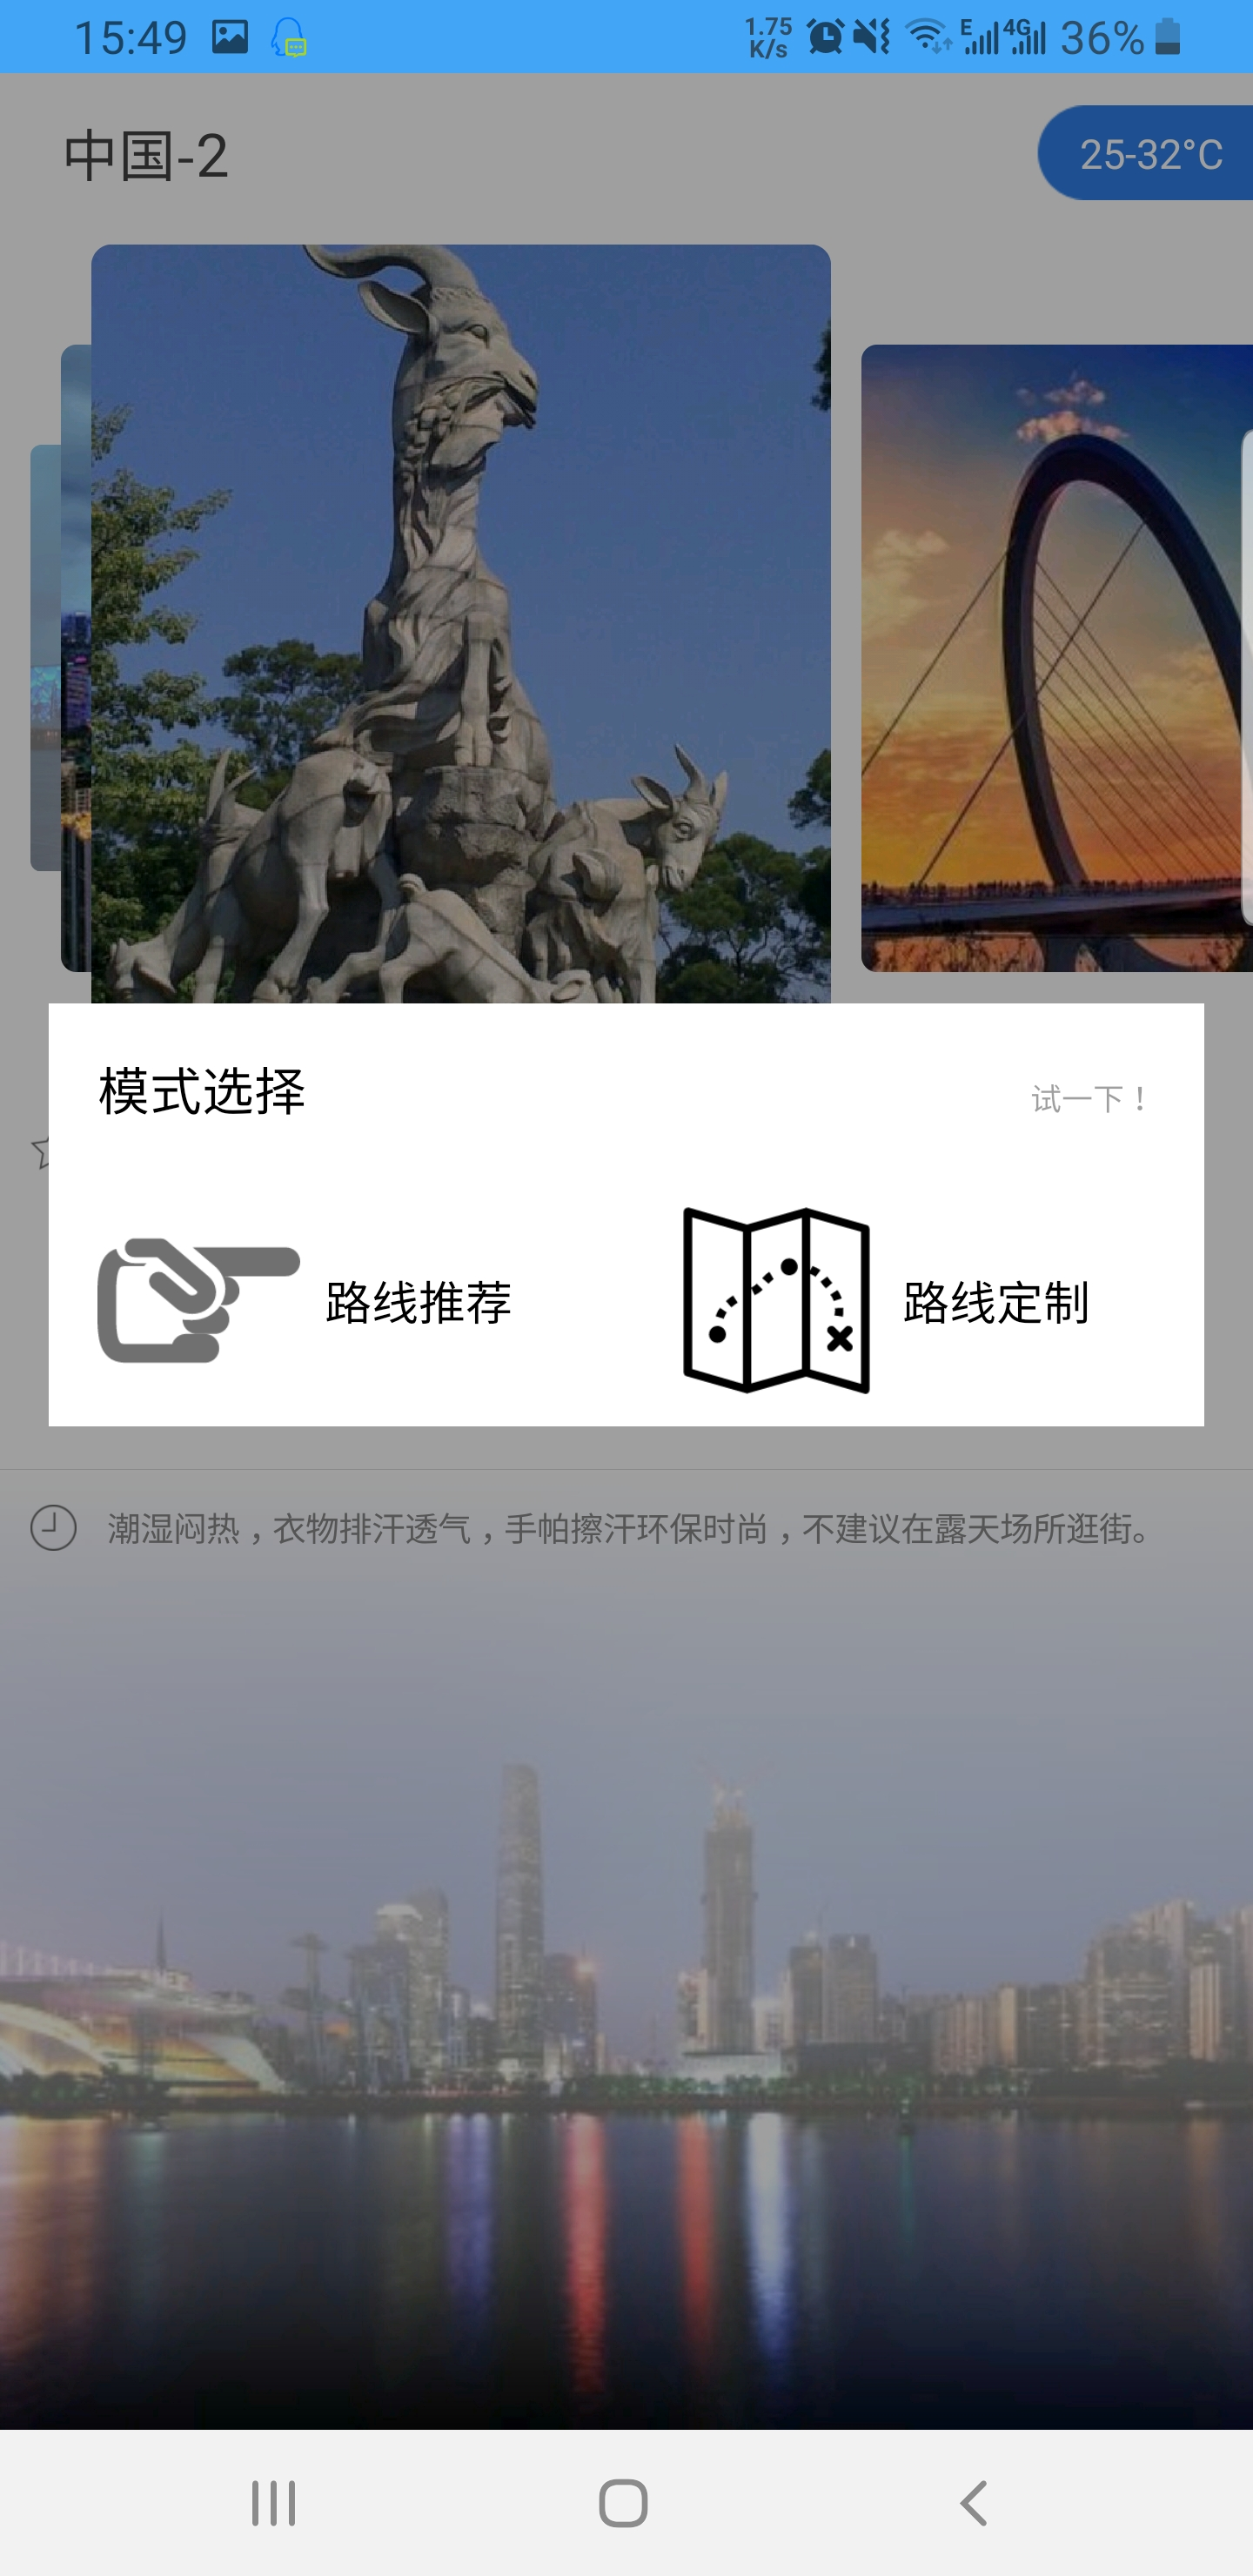
\includegraphics[width=6cm]{mode.jpg}}

	% \caption{Login}
	% \label{Login}
\end{figure}

\subsubsection{Set Preference for Recommendation}
Choose recommendation for an example. In recommendation page, we could adjust weights of  6 aspects.

Take an example, if we are like to enjoy the best acclaimed attractions, Journey Assistant may recommend us with the most popular attractions,just like BaiYun Mountain in Guangzhou as below.

\subsubsection{Display Recommendation}
Take an example, if we are like to enjoy the best acclaimed attractions, Journey Assistant may recommend us with the most popular attractions,just like BaiYun Mountain in Guangzhou as below.

Click the LIKE icon in the right bottom will add this itinerary into our liked itinerary list.

\begin{figure}[H]
	\centering
	\subfigure[Set Preference for Recommendation]{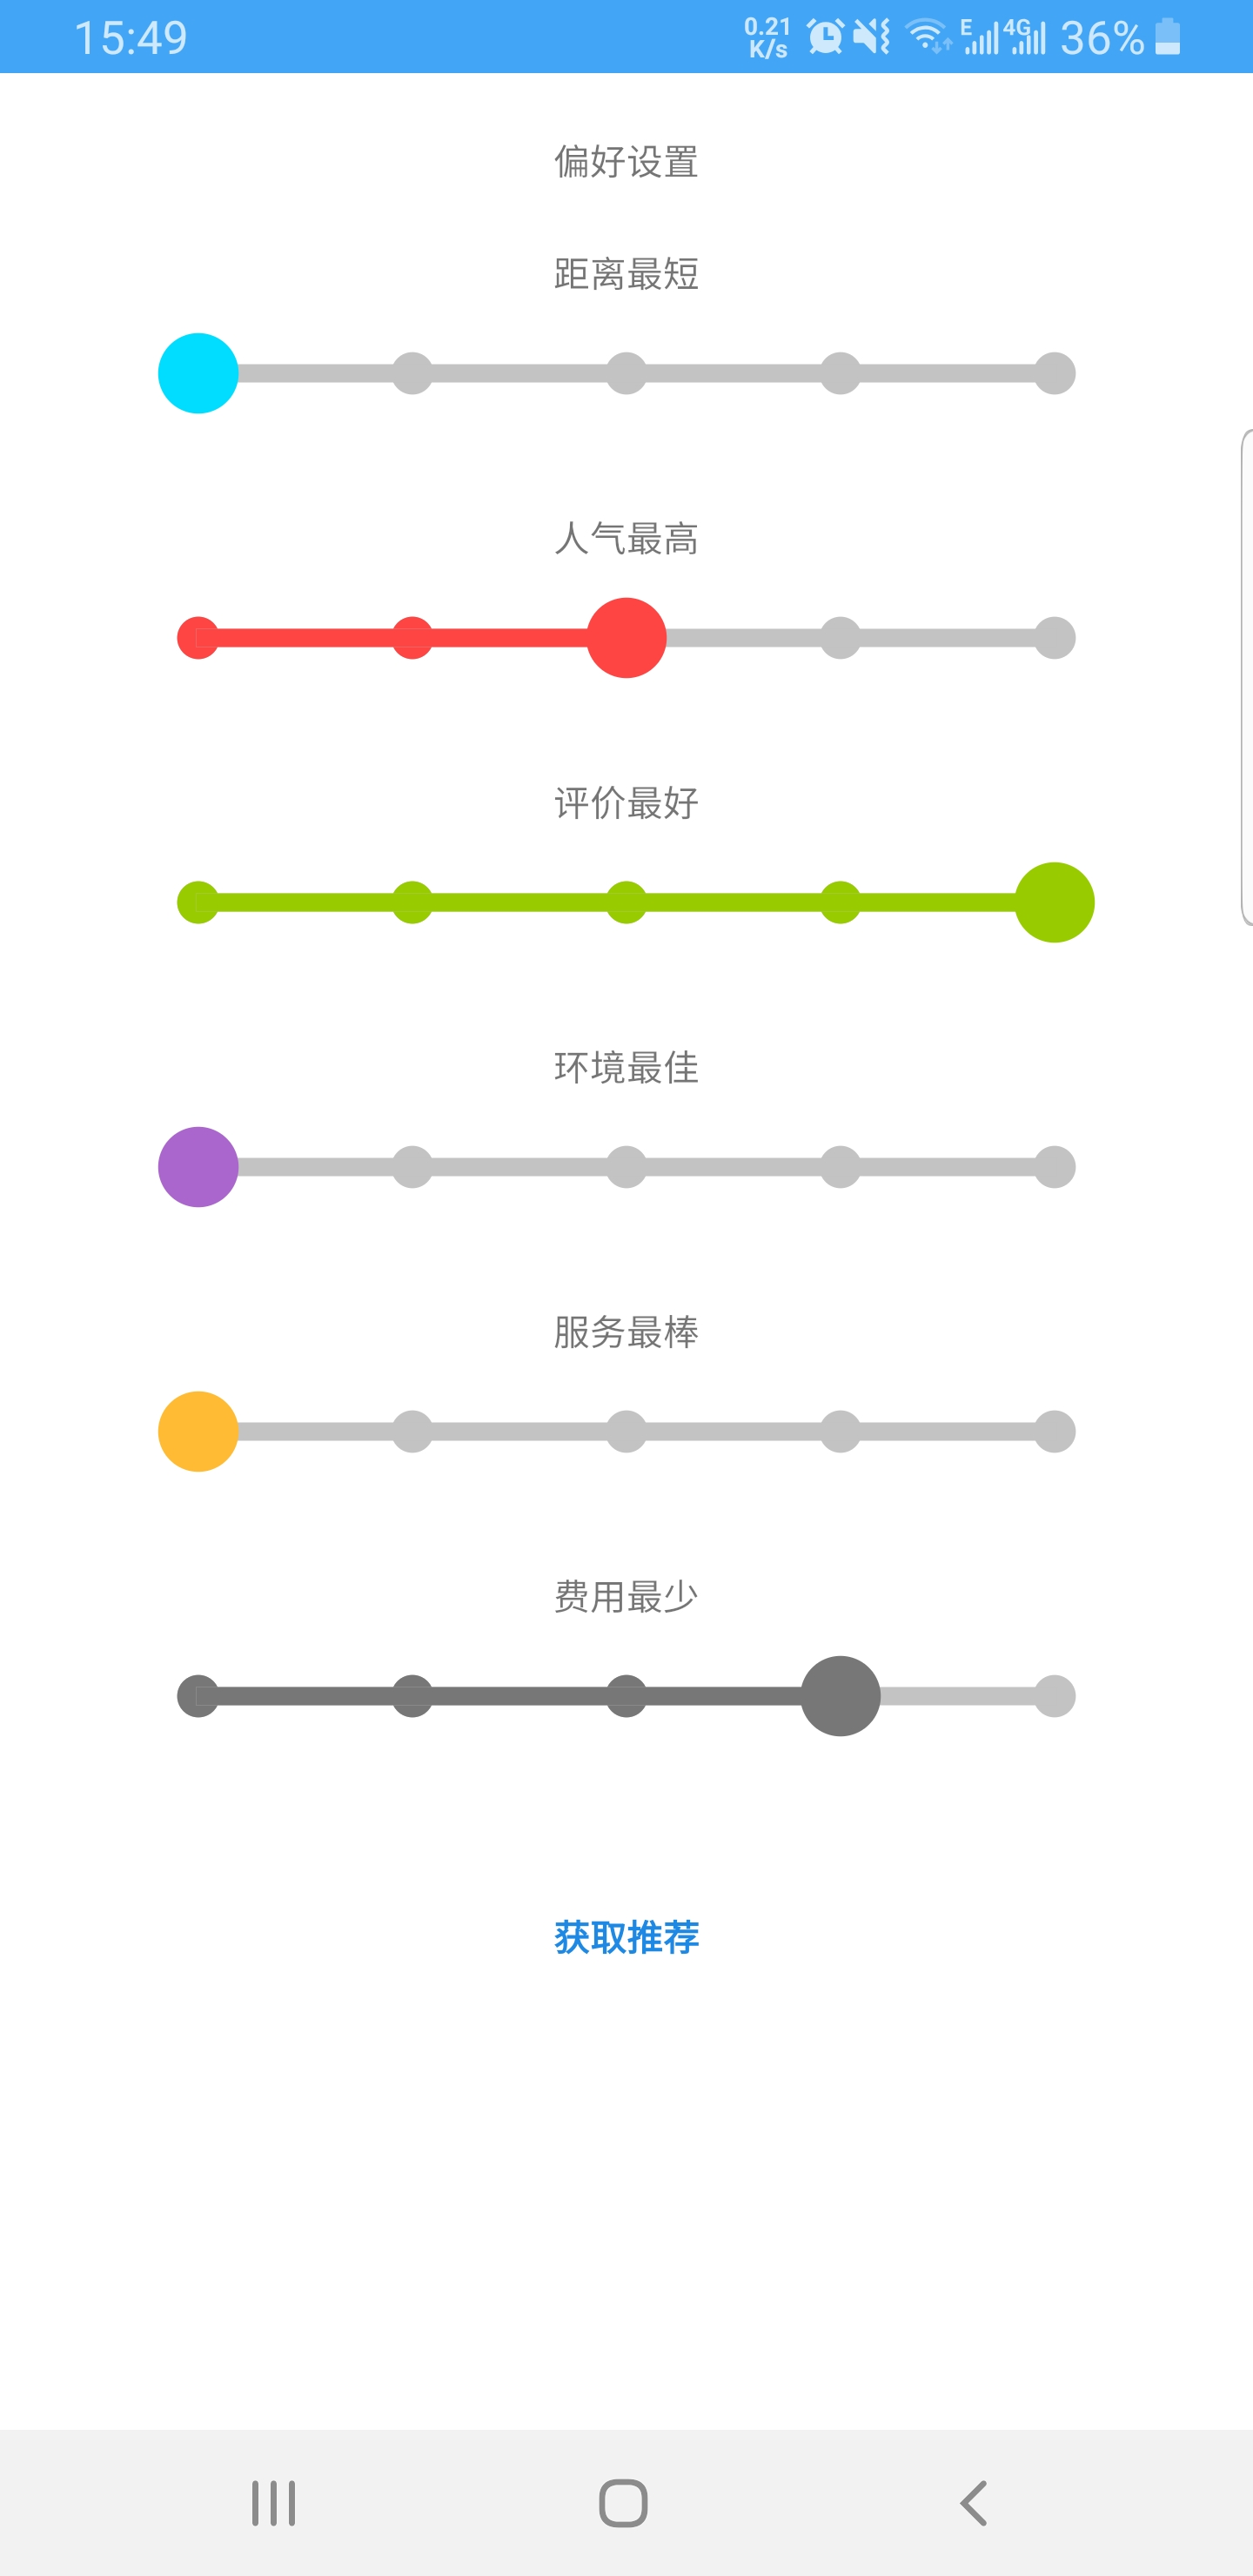
\includegraphics[width=6cm]{preference.jpg}}
	\quad
	\subfigure[Display Recommendation]{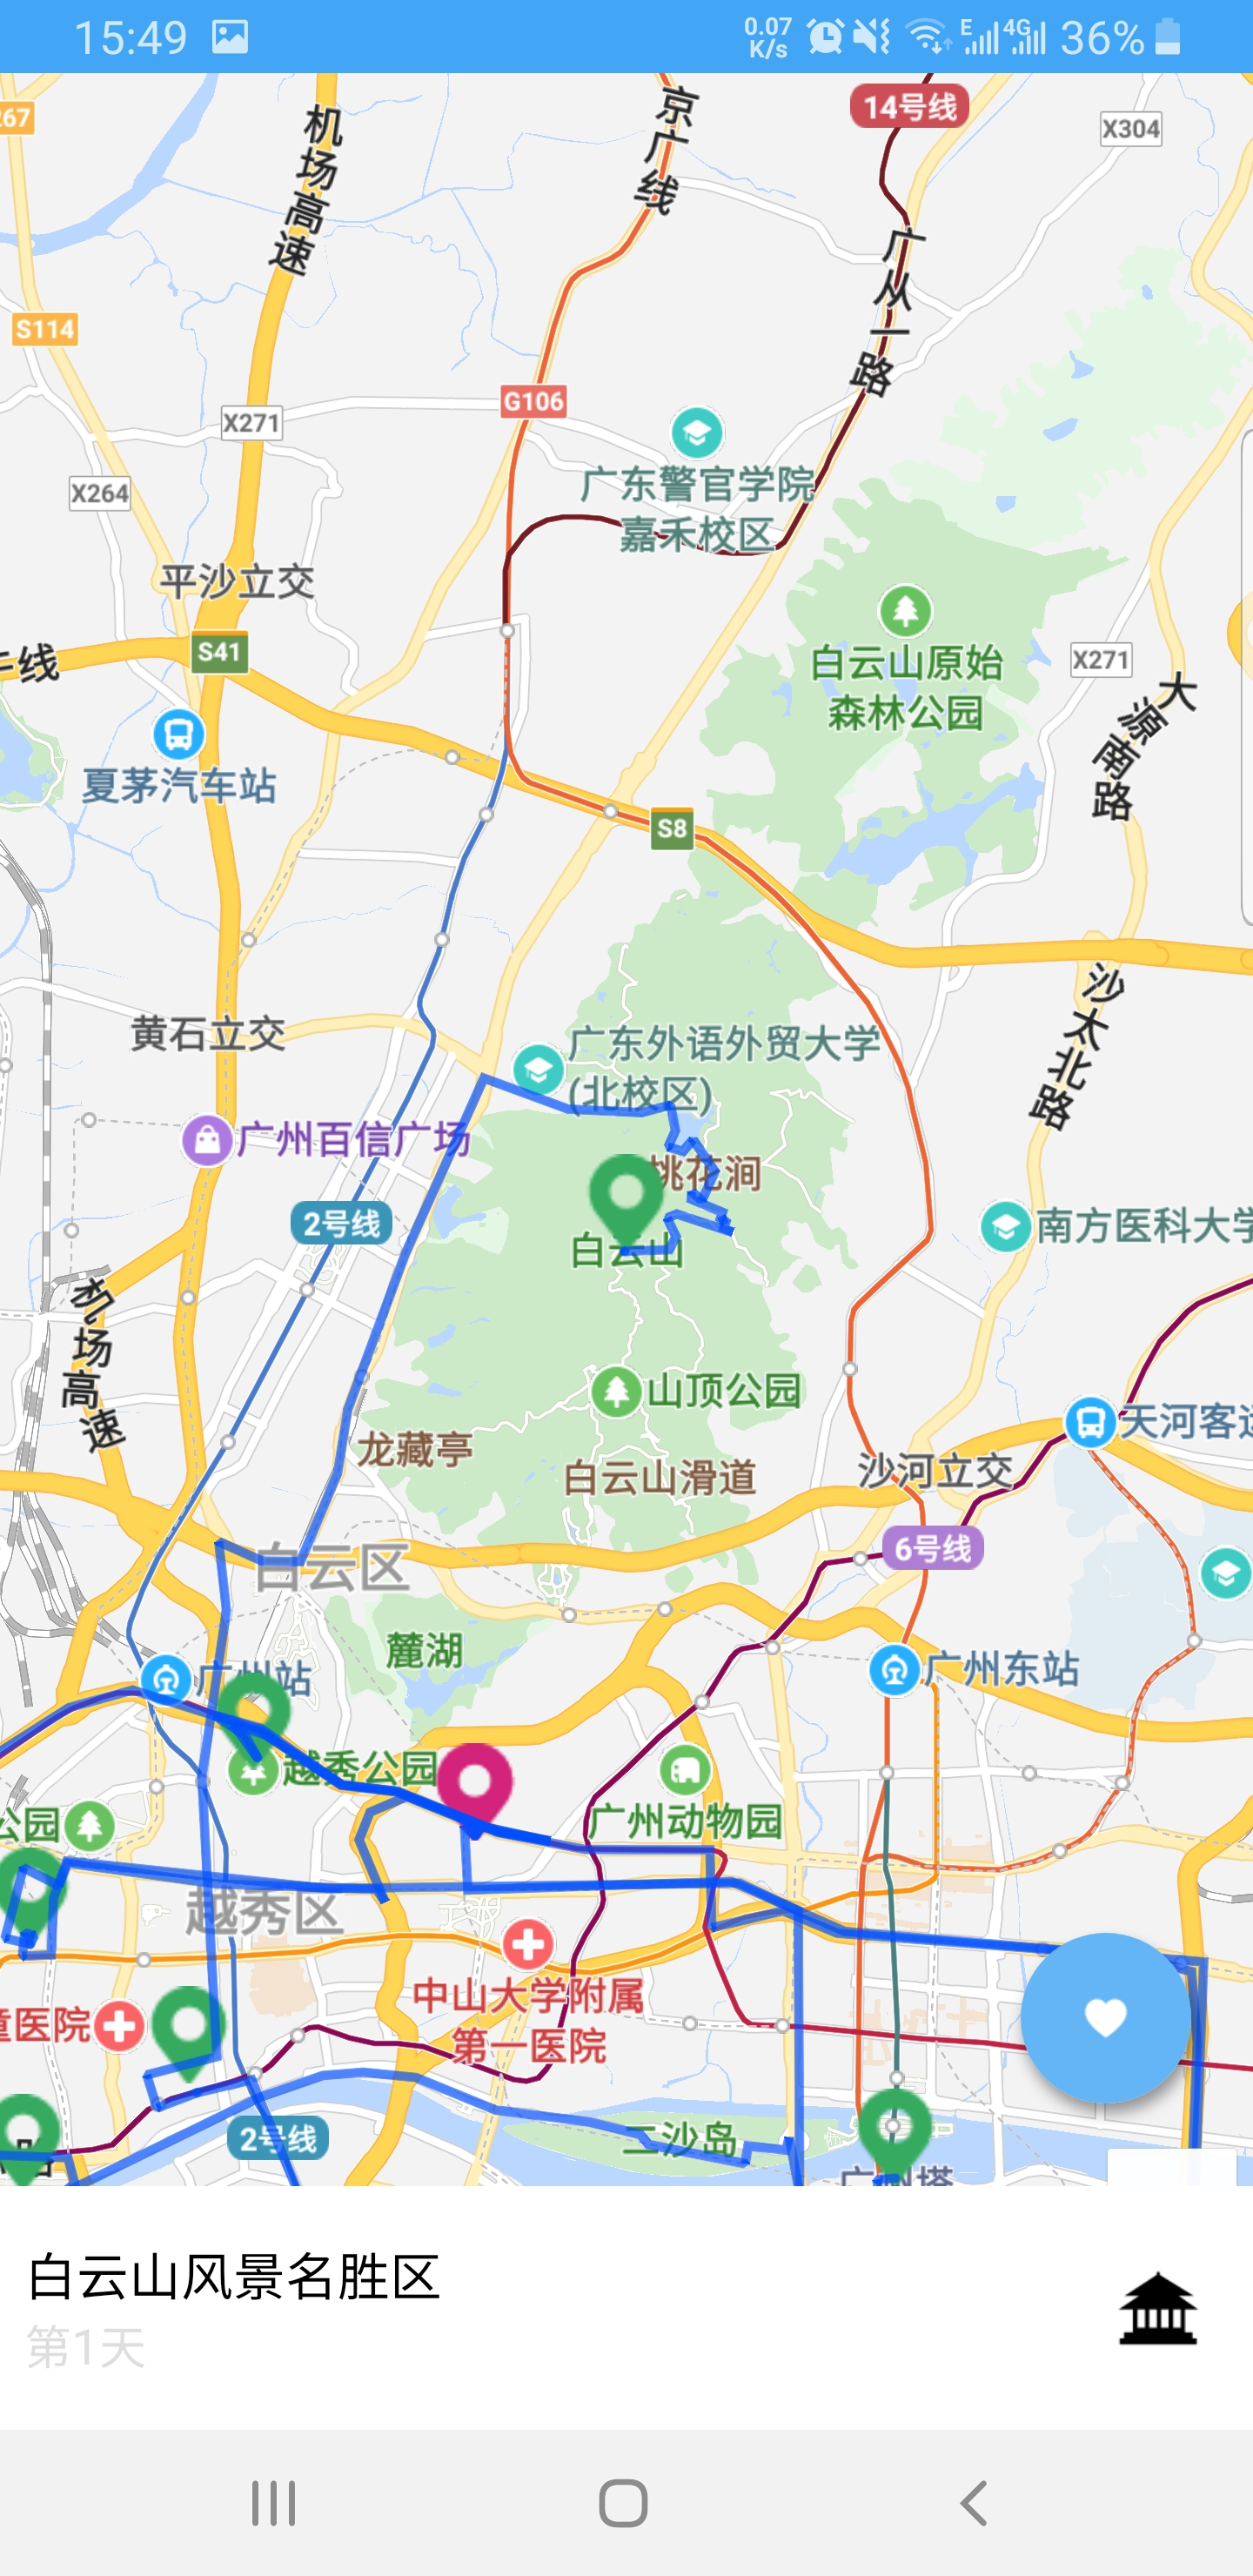
\includegraphics[width=6cm]{recommendation.jpg}}

	% \caption{Login}
	% \label{Login}
\end{figure}

\subsubsection{Customization}
Meanwhile, we could also choose itinerary by customization. In this mode,we could choose attration one by one.Once we click the icon of one attraction or hotel, basic information including Wordcloud will show up. And same as recommendation, we could also click the love icon to put it into our travel list which we will introduce in next step.

\begin{figure}[H]
	\centering
	\subfigure[Customization]{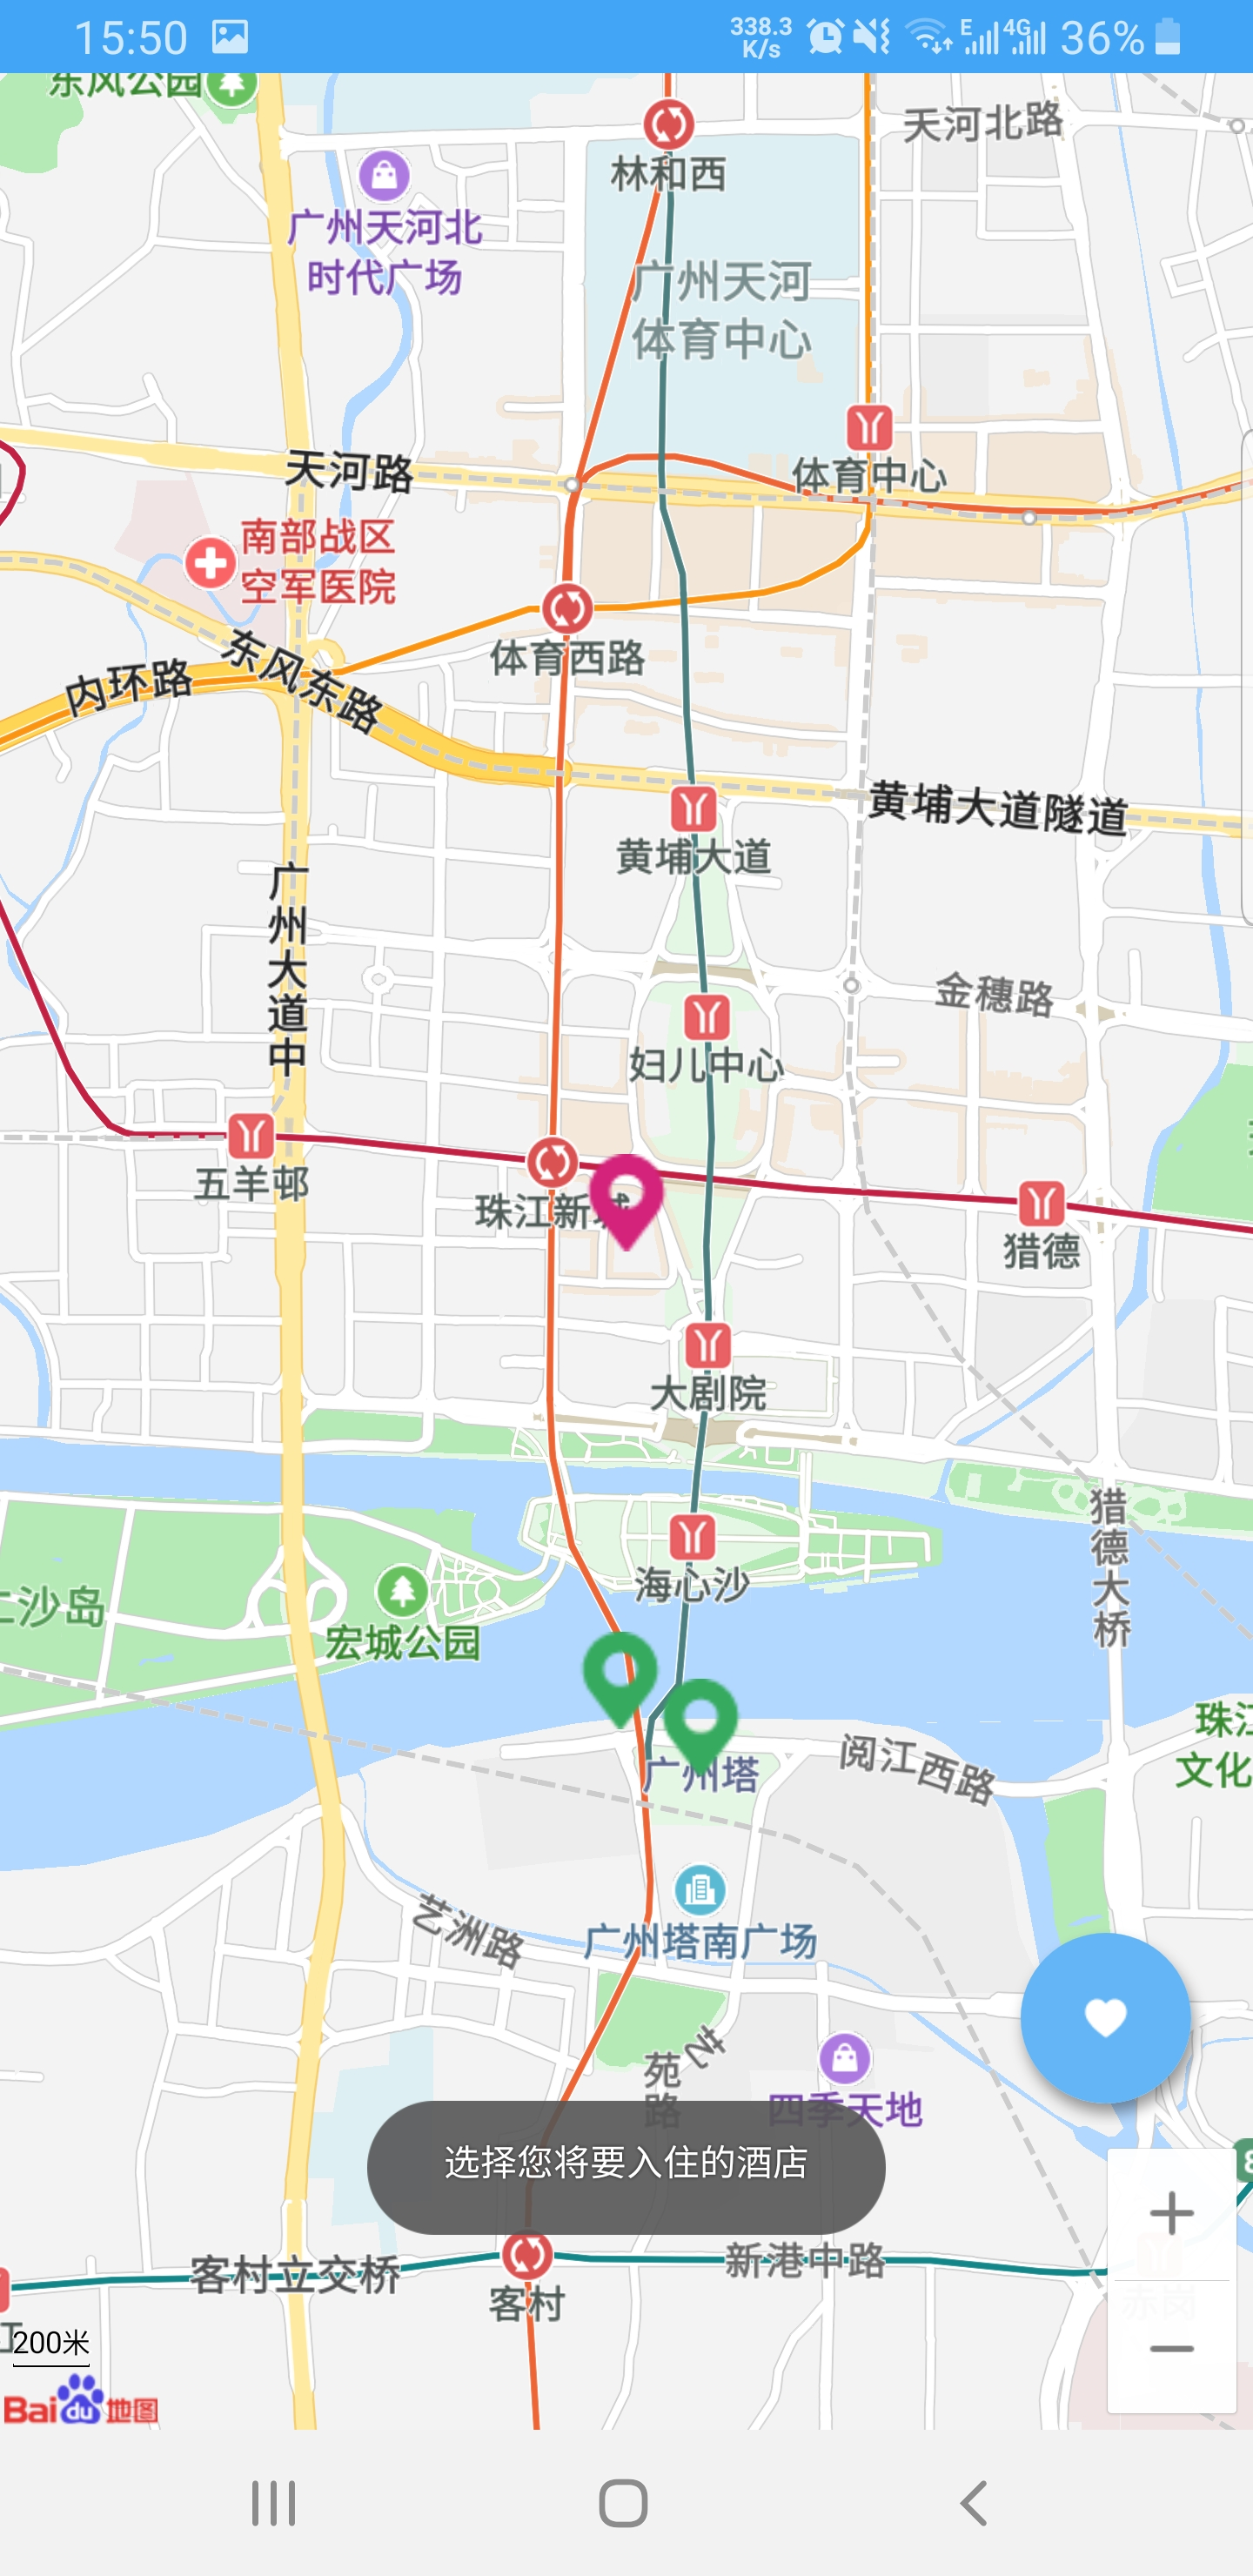
\includegraphics[width=6cm]{customization.jpg}}
	\quad
	\subfigure[Wordcloud]{\includegraphics[width=6cm]{Wordcloud.jpg}}

\end{figure}

\subsubsection{Check Itinerary List}
In the home page, we can find that there is one navigation view which can be drag from the left. We can cancel our login and read our list. In our list view, Basic Information of our itineraries confirmed before will be shown. And we could also click this cards to the correspoding city in Baidu Map. 

\begin{figure}[H]
	\centering
	\subfigure[Navigation]{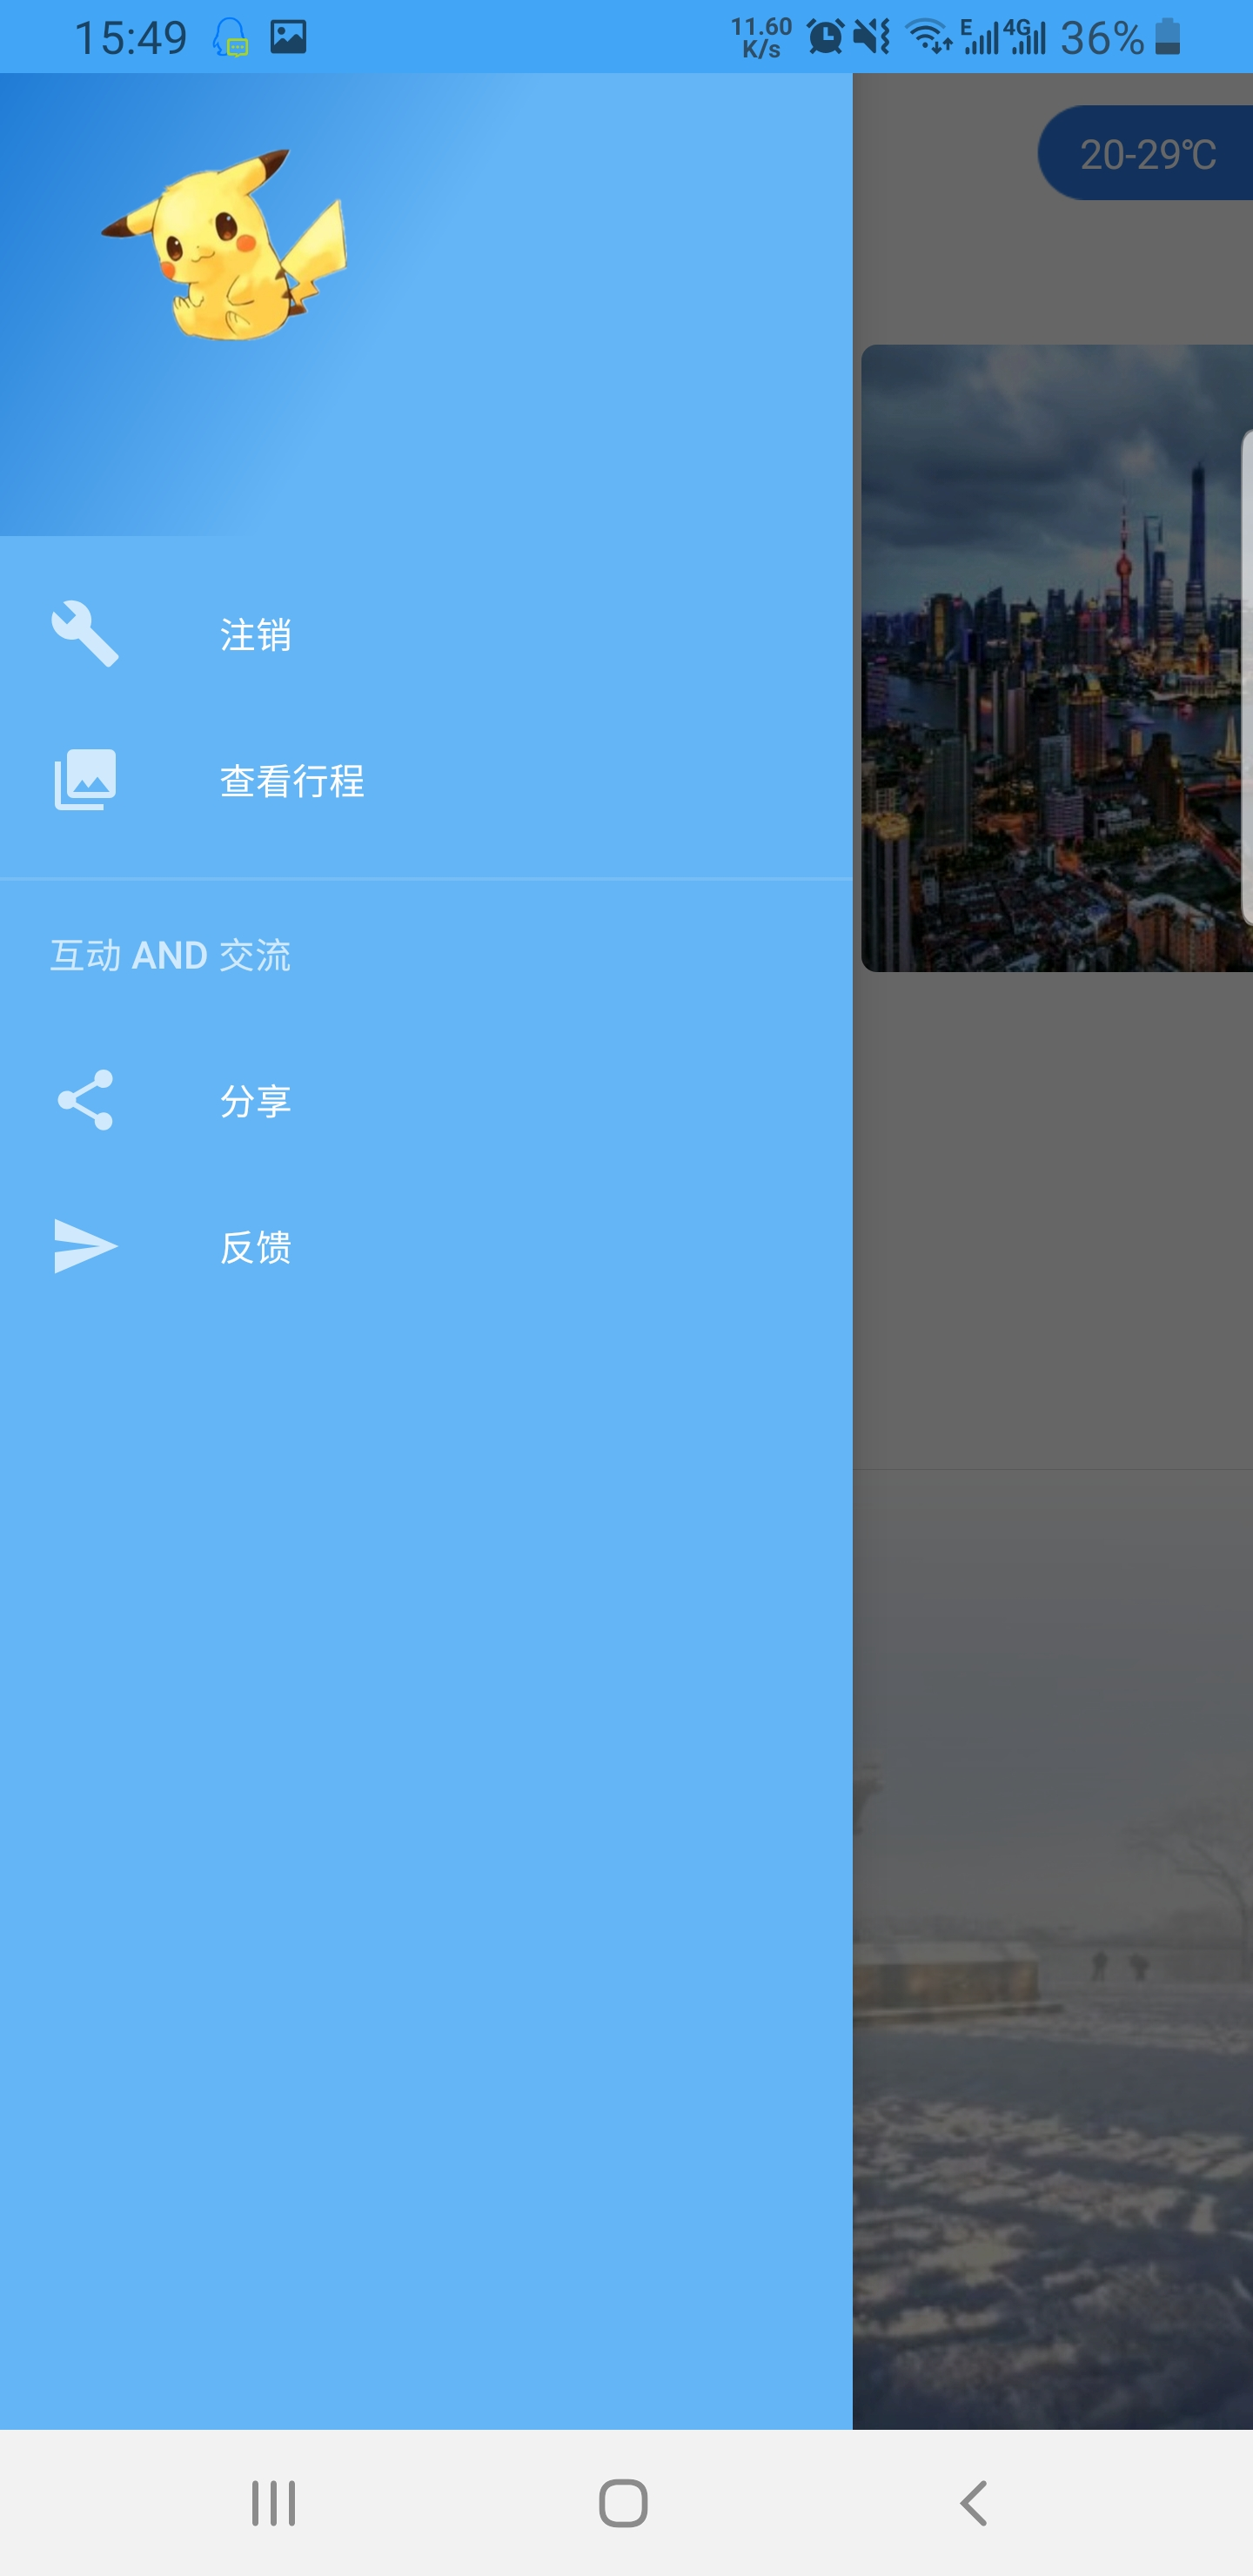
\includegraphics[width=6cm]{nav.jpg}}
	\quad
	\subfigure[Liked Itinerary]{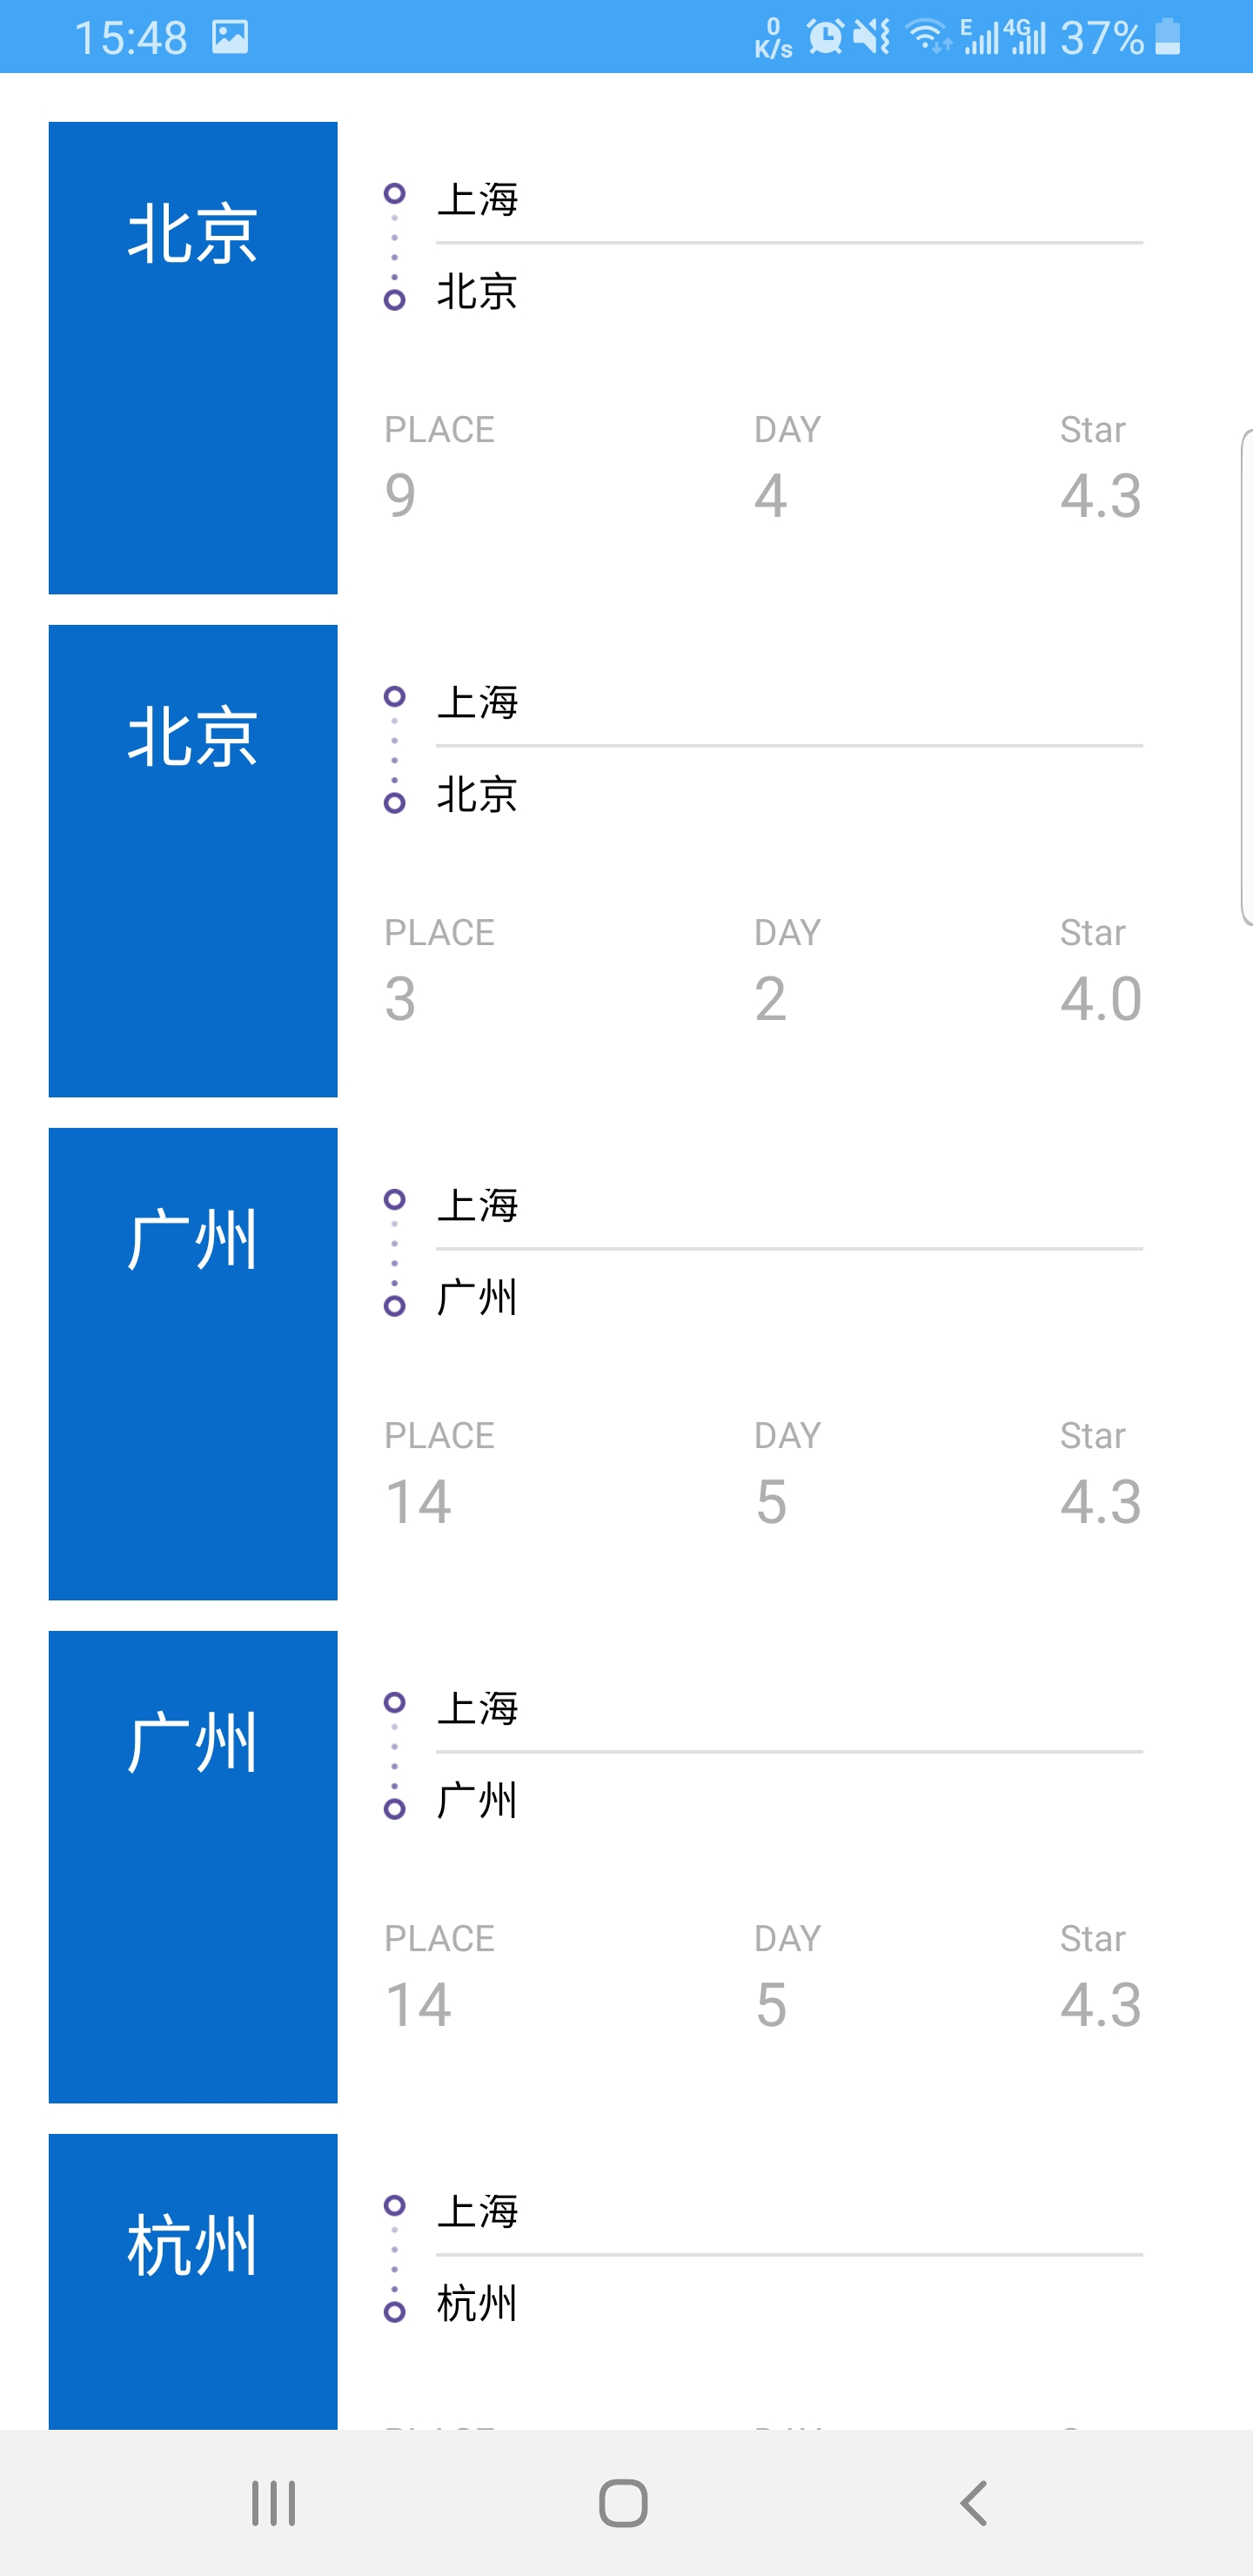
\includegraphics[width=6cm]{list.jpg}}

\end{figure}

\subsubsection{Feedback}
If we have some suggestion, we could also hand in to the developer in feedback page. On below page, we could get a screenshot of this app and put some description about the error. Clicking send button, the information will be send to us by email.

\begin{figure}[H]
	\centering
	\subfigure[Feedback]{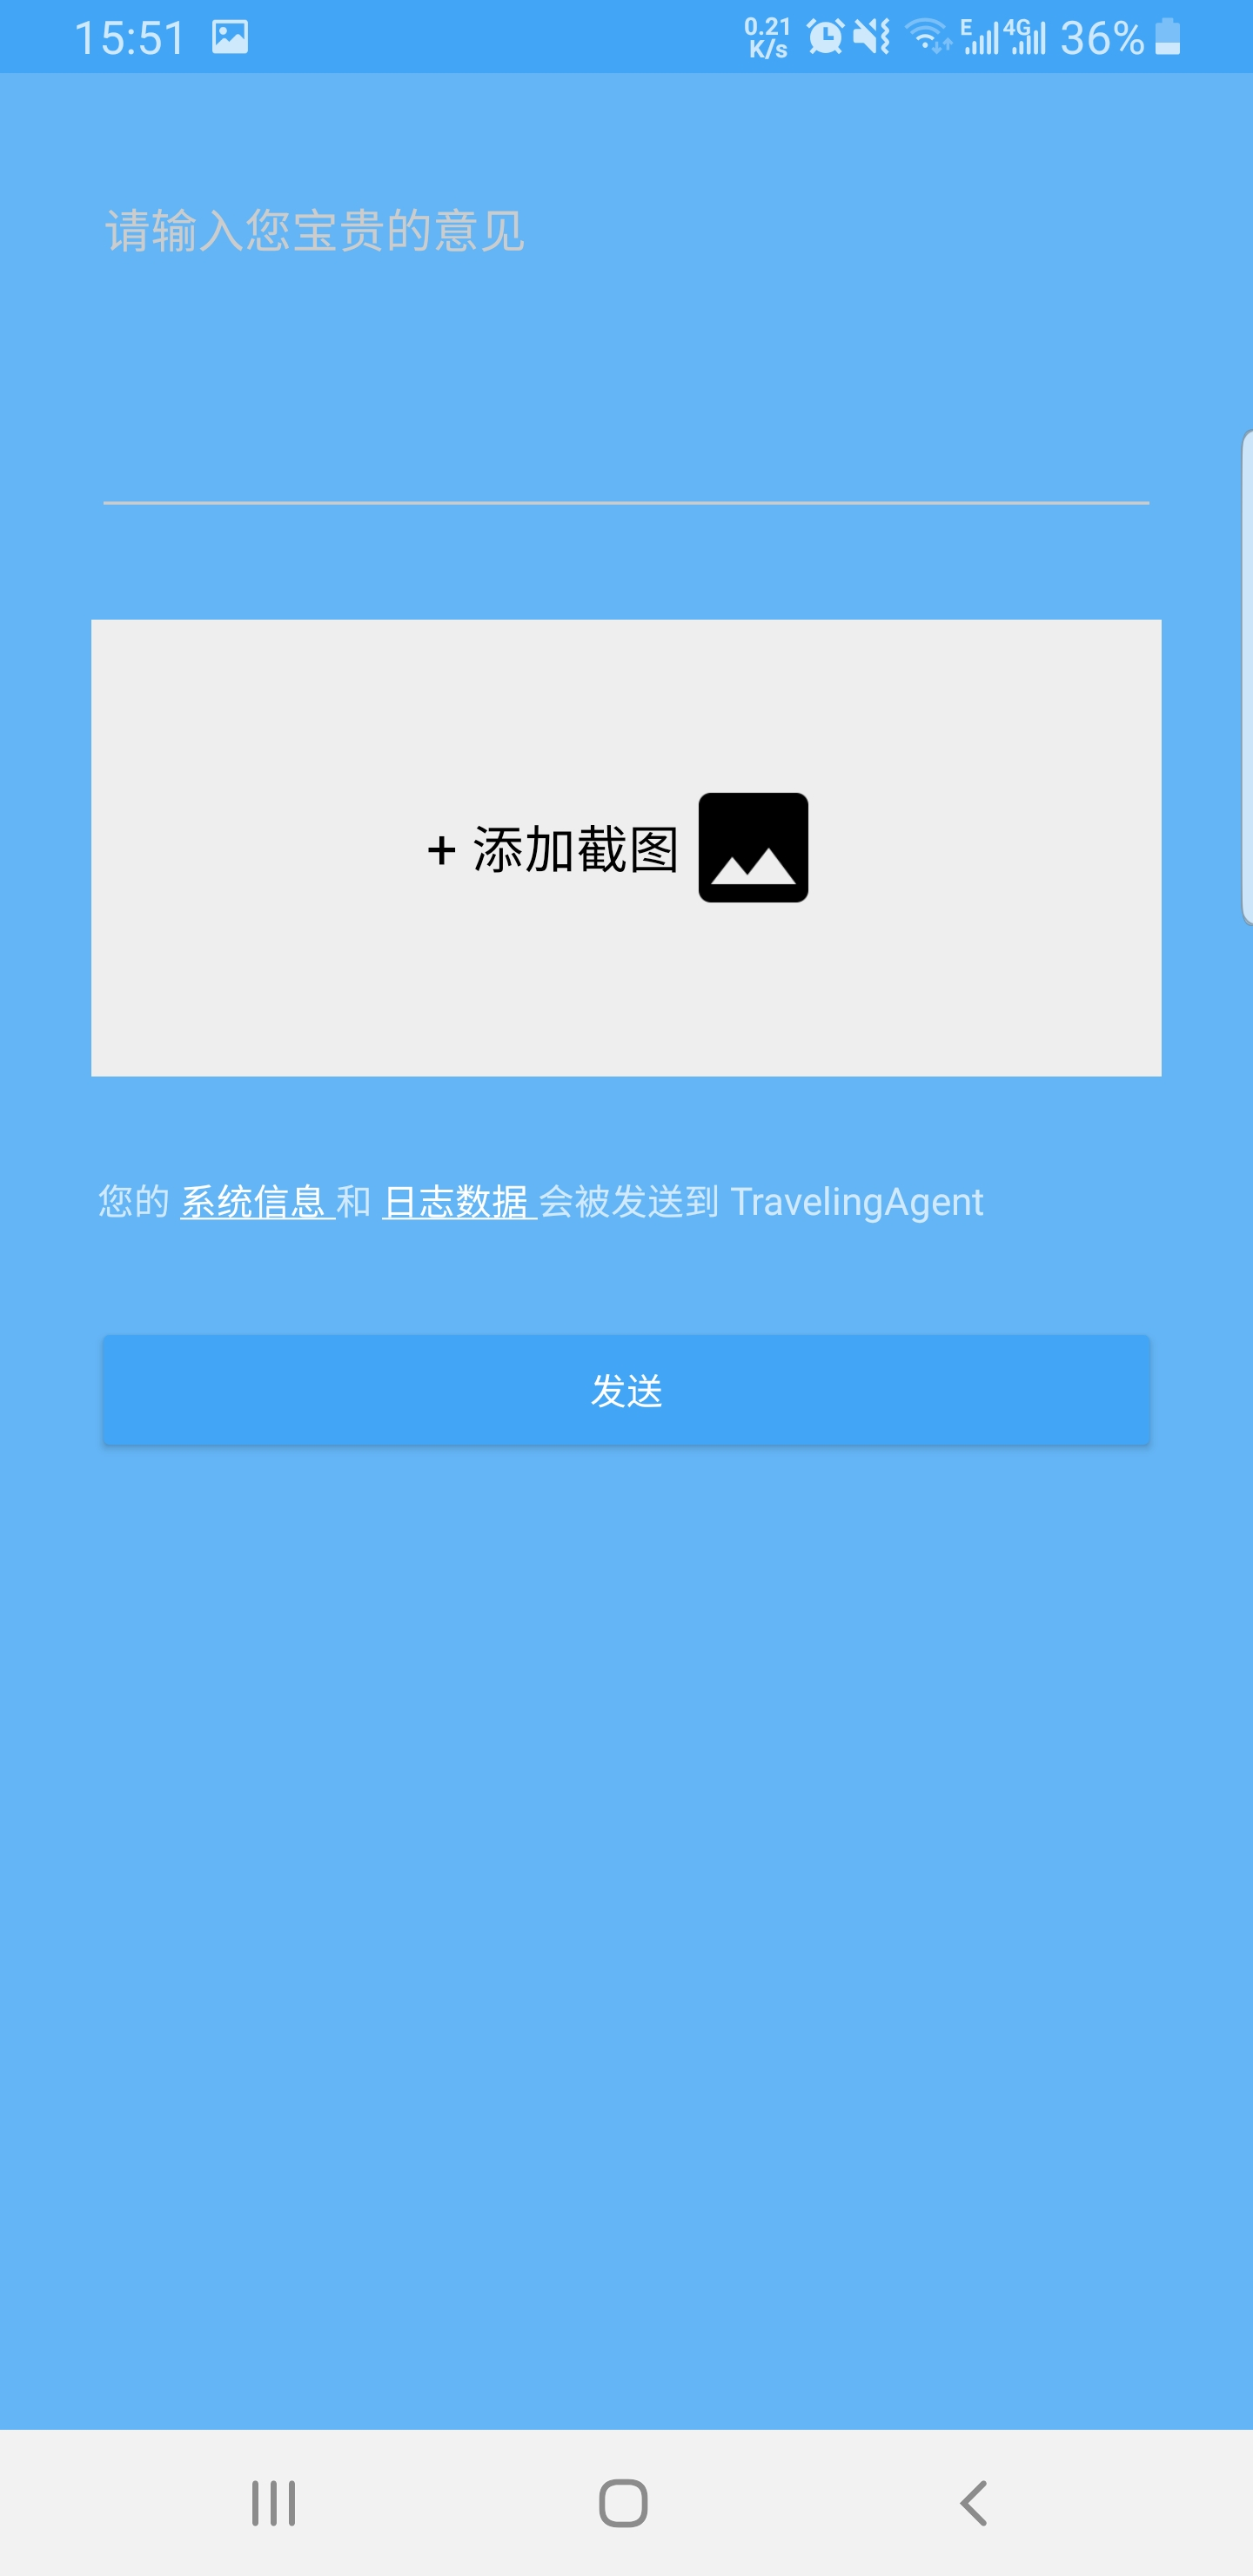
\includegraphics[width=6cm]{feedback.jpg}}

\end{figure}

\subsection{Unconventional Process}
Client run time if there is a jam, crash, etc., can restart the program. If you encounter problems while running, it is recommended to restart the server first. Contact development and maintenance staff in case of any questions or exceptions.

\end{document}
